\chapter{Data}
\label{ch:data}

\section{The Dual-Dataset Strategy}
\label{sec:dual_dataset}

Deep learning models need a lot of labeled examples to train well. A model with millions of parameters, such as a CNN-LSTM, can only learn general patterns if it sees enough varied examples of those patterns during training. Real tipping points do not give us that. They are rare by definition, and the physical sediment records that capture one -- such as a sapropel event in the Mediterranean Sea -- are scarce, hard to collect, and there is no way to know in advance which mathematical type of bifurcation actually produced any single one of them.

If we tried to train a classifier directly on the small number of real sediment cores available, it would not learn the general shape of a critical transition. It would simply memorize the noise pattern of the handful of cores it saw. This is a data bottleneck, and it rules out training directly on real geological data.

\subsection{Solution: Train on Simulation, Test on Reality}

This thesis solves the bottleneck the same way \citet{bury2021} did: split training and testing into two completely separate stages, using two different datasets.

\textbf{Training} uses \citet{bury2021}'s own synthetic dataset, released on Zenodo (Section~\ref{sec:sde_corpus} gives the exact source and how this thesis reads it). It contains hundreds of thousands of time series, each generated by numerically simulating a stochastic differential equation (SDE) that is slowly pushed toward one of three bifurcation types, or left alone as a stable control case. Because Bury et al. generated this data by simulation rather than collecting it, every label is known exactly: which bifurcation type it is, and exactly how many steps remain until the tipping point. This gives the model a large, perfectly labeled training set to learn the general statistical signature of an approaching transition -- this thesis does not generate any of it itself.

\textbf{Testing} uses real sediment cores from the PANGAEA data repository, described in Section~\ref{sec:pangaea_data}. After training finishes, every model's weights are frozen -- no further training happens on real data. The frozen model is then applied to the real cores exactly as it was applied to synthetic test data. If a model trained only on synthetic mathematics can still detect a transition in real, noisy, physical measurements it has never seen anything like before, that is real evidence the model learned something general about tipping points, not just about the synthetic dataset.

This is \citet{bury2021}'s own strategy, not an original one: they trained the same way, on synthetic data alone, and tested the frozen result on real records they never trained on. This thesis follows it directly, extending it to a much larger set of model architectures (Chapter~\ref{ch:methodology}).

\section{Synthetic Training Data: The SDE Corpus}
\label{sec:sde_corpus}

\subsection{Four Classes, and What Actually Generates Them}

The synthetic dataset has four classes: fold, transcritical, and Hopf bifurcations, plus a null (no-transition) control class. Chapter~\ref{ch:theoretical_background} derives the canonical normal form for each of these -- the simplest possible equation of that bifurcation type:

\begin{align}
    \text{Fold: }\quad          & dx = (\lambda - x^2)\, dt \\
    \text{Transcritical: }\quad & dx = (\lambda x - x^2)\, dt \\
    \text{Hopf: }\quad          & dr = (\lambda r - r^3)\, dt, \quad d\theta = \omega\, dt
\end{align}

It is important to be precise about what these equations are and are not. They are \emph{not} the literal equations that \citet{bury2021} numerically integrated to produce each training series. The actual generator, confirmed directly against the data-generation code in their public repository \citep{burygithub}, is a randomly-parameterized two-dimensional cubic polynomial system,
\begin{equation}
    \frac{dx}{dt} = \sum_{k=1}^{10} a_k\, \phi_k(x,y), \qquad
    \frac{dy}{dt} = \sum_{k=1}^{10} b_k\, \phi_k(x,y),
\end{equation}
where $\phi_k$ runs over the ten monomials $1, x, y, x^2, xy, y^2, x^3, x^2y, xy^2, y^3$ and the twenty coefficients $a_k, b_k$ are drawn at random (about half of them set to zero) for every candidate system. Each candidate is then checked with bifurcation-continuation software (AUTO) to see whether, as one of its coefficients is varied, it passes through a fold, a transcritical (called a "branch point" in their code), or a Hopf bifurcation; systems that do not are discarded. Only systems that pass through the target bifurcation type are kept and simulated.

The canonical normal forms in Chapter~\ref{ch:theoretical_background} still matter here, but for a specific mathematical reason and not because they were simulated directly: the Normal Form Theorem guarantees that \emph{any} system near a generic fold, transcritical, or Hopf bifurcation behaves, close enough to the bifurcation point, exactly like its canonical normal form. That is precisely why a classifier can be trained on this library of many different random polynomial systems and still learn one consistent signature per bifurcation type -- every system in the fold class is locally equivalent to the fold normal form near its own tipping point, even though the full polynomial equation differs from series to series. This library-of-random-systems approach, rather than simulating one fixed equation per class, is also why the training set contains far more genuine variety than four equations would suggest, and it is a deliberate design choice on Bury et al.'s part: reducing the risk that a classifier just memorizes one specific equation's noise profile instead of the general shape of critical slowing down.

For the Hopf class, only the $x$ component of the two-dimensional system is kept as the training series. Every other class already produces one usable series directly. The null class is generated the same way, except the varying coefficient is held fixed at a point away from any bifurcation, so the system stays permanently stable. It matters as much as the other three classes: without it, a model would learn to flag \emph{any} noisy series as a coming transition, since every training example it ever saw would be building towards one.

\subsection{Generating the Series}

Every series -- for all four classes -- is produced with the Euler-Maruyama method, the standard way to turn a continuous stochastic differential equation into a discrete sequence a computer can generate step by step, confirmed directly against \citet{burygithub}'s simulation code. Two things vary across the dataset:

\begin{itemize}
    \item \textbf{Noise amplitude} is not a flat random draw. It is computed per series as $\sigma = \sqrt{2\gamma}\,\tilde{\sigma}\,\xi$, where $\gamma$ is the system's own local recovery rate near its starting point, $\tilde{\sigma}=0.01$ is a fixed base amplitude, and $\xi$ is a triangularly-distributed random variate. Scaling the noise by the recovery rate means systems that relax back to equilibrium slowly (and are therefore closer to a bifurcation to begin with) are not accidentally given disproportionately large noise, keeping the amount of critical slowing down present in the data controlled rather than arbitrary.
    \item \textbf{Forcing}: for the three bifurcation classes, the varying coefficient is moved linearly in time from its starting value to the exact value at which AUTO located the bifurcation, so every series in a class ends at its own version of the same bifurcation type. In the null class this coefficient never moves.
\end{itemize}

Every simulation also runs a 100-time-unit burn-in period at the start, which is thrown away before recording begins. This removes the influence of the arbitrary starting point, so what remains is the system settling into its own dynamics, not an artifact of how the simulation happened to be initialized.

This thesis does not run any of the simulation described above itself -- it downloads Bury et al.'s already-generated dataset from Zenodo and reads it directly (\texttt{src/preprocess\_bury\_data.py} repackages their released \texttt{labels.csv}, \texttt{groups.csv}, and per-series residual files into the format used for training). The description above is included because understanding how the training labels were actually produced -- a library of varied random systems rather than four fixed equations -- matters for correctly interpreting what a trained classifier has learned.

\subsection{Two Sequence Lengths}

\citet{bury2021} released classifiers trained at two fixed lengths, $L=500$ and $L=1500$ (Chapter~\ref{ch:related_work}, Section~\ref{sec:bury2021}). This thesis uses both lengths too, across every model in the full model suite of Chapter~\ref{ch:methodology}, not just the original CNN-LSTM. Comparing the two lets us check whether a longer input window -- which gives a classifier more data points to estimate a slow variance ramp from -- actually helps.

It does, but the effect is smaller and more model-dependent than a single number suggests. Averaged across all 19 models with results at both lengths, moving from $L=500$ to $L=1500$ raises macro-AUC (one-vs-rest, Chapter~\ref{ch:methodology}, Section~\ref{sec:evaluation_metrics}) by 3.6 percentage points at the median. The strongest gains all belong to classical time series classifiers: rdst (+7.3), mrsqm (+6.2), and rocket (+6.1). The weakest gains are inceptiontime and weasel2 (both +0.8), with lstm and tcn close behind (+1.7) -- these four were already close to their ceiling at $L=500$. One model, MultiRocket, actually performs \emph{worse} at $L=1500$ ($-$9.7 points) -- a reminder that a longer window is not automatically better for every architecture, and that this needs checking per model rather than assumed.

\section{Empirical Test Data: PANGAEA Mediterranean Sediment Cores}
\label{sec:pangaea_data}

\subsection{Sapropels as Real Tipping Points}

The Mediterranean Sea has repeatedly gone through sapropel events: periods where the deep water loses essentially all of its dissolved oxygen, and a dark, organic-rich layer of sediment is deposited on the seafloor as a result. These events are driven by slow changes in Earth's orbit that intensify the African monsoon, which increases freshwater runoff into the Mediterranean. That freshwater sits on top of the denser seawater and blocks the vertical mixing that normally carries oxygen down to the seafloor.

Whether this represents a slow, proportional response to orbital forcing, or a genuine tipping point, is exactly the kind of question this thesis's method is built to test. \citet{hennekam2020} already applied classical early-warning-signal methods to these same records: rising variance and lag-1 autocorrelation, using the sliding-window approach described in Chapter~\ref{ch:related_work}, Section~\ref{sec:classical_method}. They found strong signals in the two deepest cores and almost none in the shallowest one (Chapter~\ref{ch:related_work}, Section~\ref{sec:hennekam_ews} gives the depth-dependent result in full). That result does not by itself prove a bifurcation occurred, and it says nothing about which \emph{type}. This thesis's contribution is to test that more rigorously with the trained classifiers from Chapter~\ref{ch:methodology}, and to attempt to diagnose the bifurcation type.

We use three sediment cores originally compiled by \citet{hennekam2020}: MS21, MS66, and 64PE406E1. These are the same cores \citet{bury2021} used as their own empirical test case, via the same PANGAEA dataset (DOI 10.1594/PANGAEA.923197), confirmed directly in their code repository's own README \citep{burygithub}.

\subsection{The Five Geochemical Proxies}

Each core is measured at millimeter resolution for five chemical elements, following \citet{hennekam2020}. Proxy interpretations follow \citet{tribovillard2006}:

\begin{itemize}
    \item \textbf{Molybdenum (Mo) and Uranium (U) -- redox proxies.} Both metals stay dissolved in normal, oxygenated seawater. Once the water column turns anoxic, they precipitate out and accumulate in the sediment. A sharp rise in Mo or U is the direct chemical signature that anoxia has actually set in -- these are the two proxies most directly tied to the event itself.
    \item \textbf{Barium (Ba) -- productivity proxy.} Nutrient-rich river runoff before a sapropel drives plankton blooms; the sinking organic matter concentrates biogenic barium in the sediment as it decays. Barium can also be affected by how well barite is preserved under changing oxygen conditions, so it is a noisier proxy than Mo or U.
    \item \textbf{Titanium (Ti) and Aluminum (Al) -- terrestrial input proxies.} These come from windblown dust and river sediment, not from the ocean chemistry itself. They track the strength of the monsoon rains that are the actual driver of the whole process -- closer to a proxy for the forcing parameter than for the transition.
\end{itemize}

All five elements are cleaned and reconstructed the same way (\texttt{src/pangea\_cleaner.py}). The PANGAEA evaluation itself, however, uses only Mo and U (\texttt{src/rolling\_window.py}): the two proxies tied directly to the redox transition, rather than to its indirect drivers or to a noisier productivity signal. Chapter~\ref{ch:results}, Section~\ref{sec:pangaea_provenance} gives the full reasoning and what an earlier, now-superseded five-element evaluation showed.

\section{Verifying the Ground Truth: Correcting the Sapropel Onset Ages}
\label{sec:label_correction}

Every classifier in this thesis needs to know two things about a real sapropel to be evaluated fairly: which time window comes \emph{before} the transition (so the model can be asked "do you see this coming"), and where the transition actually is. Both depend entirely on one number per sapropel: its onset age.

\subsection{How the Ages Were Checked}

A real sapropel is not just a label -- it is a specific, measurable geochemical event: Mo and Ba concentrations rise sharply above the core's normal background level exactly when anoxia sets in (Section~\ref{sec:pangaea_data}). This makes the onset age independently checkable, by scanning the raw XRF measurements around the claimed age and asking whether the chemistry is actually elevated there.

Doing this check surfaced a serious problem. Every onset age used earlier in this project, apart from the youngest sapropel in each core (S1), was wrong by 60 to 140 thousand years. Table~\ref{tab:label_correction} shows the scale of the error for core 64PE406E1: the originally used ages sit at 0.6--1.1$\times$ the core's own background Mo level -- statistically ordinary mud, not a sapropel at all -- while the corrected ages sit at 3--27$\times$ background, which is the expected signature of a real sapropel.

\begin{table}[htbp]
\centering
\caption{Sapropel onset ages before and after correction, core 64PE406E1. Enrichment is measured relative to the core's own background median Mo concentration (2.35 mg/kg).}
\label{tab:label_correction}
\begin{tabular}{lrcrc}
\toprule
Sapropel & Original age (ka) & Mo enrichment & Corrected age (ka) & Mo enrichment \\
\midrule
S9 & 104.0 & 0.9$\times$ & 240.6 & 4.6$\times$ \\
S8 & 89.0  & 1.1$\times$ & 226.6 & 3.0$\times$ \\
S7 & 74.0  & 0.8$\times$ & 198.2 & 21.3$\times$ \\
S6 & 59.0  & 0.9$\times$ & 177.9 & 12.3$\times$ \\
S5 & 54.0  & 0.6$\times$ & 127.9 & 26.6$\times$ \\
S4 & 39.0  & 0.8$\times$ & 107.6 & 7.9$\times$ \\
S3 & 22.5  & 1.0$\times$ & 85.4  & 12.6$\times$ \\
\bottomrule
\end{tabular}
\end{table}

Figure~\ref{fig:label_correction} shows this directly on the raw Mo record for 64PE406E1. The originally used ages (dashed red lines) fall in stretches of the core with no Mo enrichment at all. The corrected ages (solid green lines) line up with the real spikes in the record.

\begin{figure}[htbp]
\centering
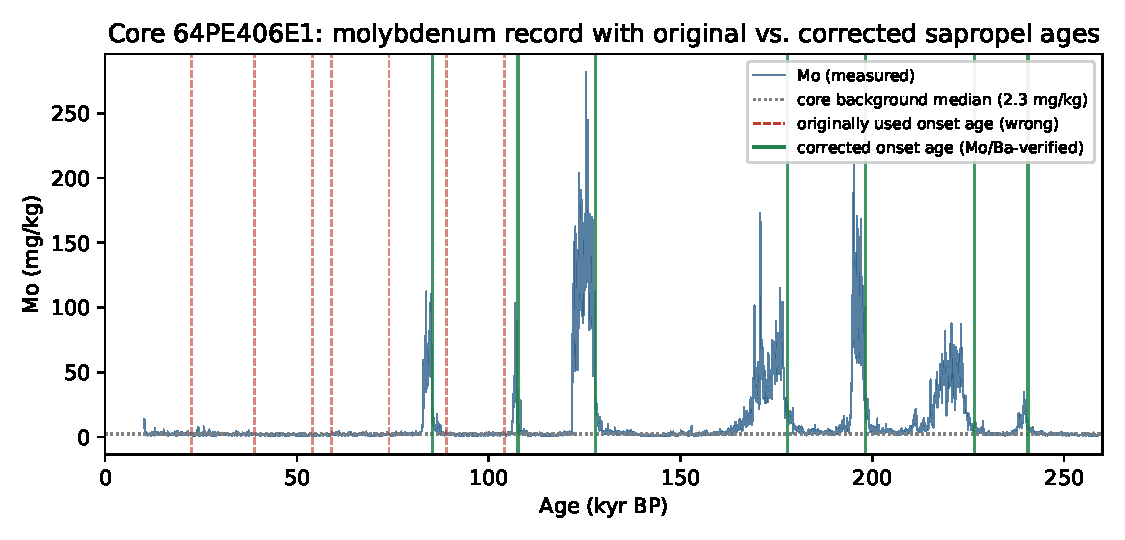
\includegraphics[width=0.95\textwidth]{figures/fig5_label_correction.pdf}
\caption{Molybdenum record for core 64PE406E1, with the originally used sapropel onset ages (dashed red) compared against the corrected, Mo/Ba-verified ages (solid green). The originally used ages do not correspond to any real geochemical enrichment.}
\label{fig:label_correction}
\end{figure}

The same pattern held across all three cores and every sapropel except S1, the youngest sapropel in each core, whose original age was already close to the Mo/Ba-verified one. This project did not investigate why S1 specifically was already accurate while the older sapropels were not; it is reported here as an observation, not an explained one.

\subsection{Why This Mattered}

Because the "before transition" windows fed to the models were cut from the wrong part of each core, they contained ordinary glacial-age sediment with no real transition in it. Evaluating a model on that data and getting a near-chance result (AUC around 0.5) is not evidence the model doesn't work -- it is the expected outcome of testing it on the wrong data.

Correcting the ages also fixed a second, related problem: the corrected sapropels turned out to be longer than the ones originally used, since the true event windows are wider than where they were mistakenly placed. Figure~\ref{fig:segment_lengths} shows this for the seven segments that changed most: real segment length grew by roughly 40\% to nearly 3$\times$ once the correct ages were used, not by a uniform multiple across sapropels. Longer real segments mean less of the model's fixed-length input window has to be padded with zeros, and less padding means the input the model sees during testing looks more like what it saw during training.

\begin{figure}[htbp]
\centering
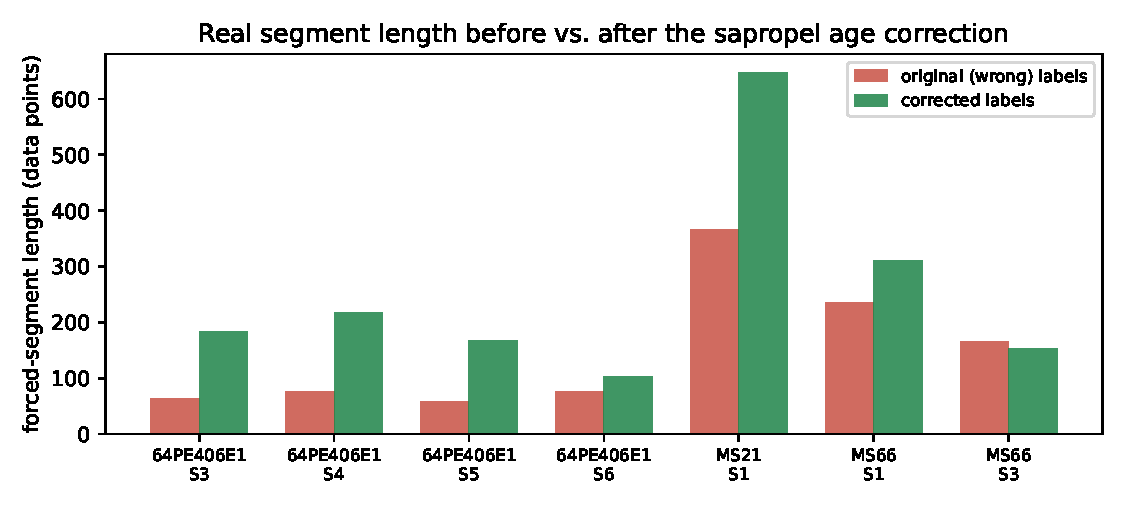
\includegraphics[width=0.95\textwidth]{figures/fig5_segment_lengths.pdf}
\caption{Length of the usable pre-transition data segment, before and after the age correction, for the seven sapropels most affected. Longer segments mean less zero-padding is needed to reach the model's fixed input length.}
\label{fig:segment_lengths}
\end{figure}

Six models (arsenal, cnn\_lstm, inceptiontime, lstm, minirocket, rocket) were evaluated on both the original and the corrected ages, before the model roster grew to its current size; this is the only part of the roster where a direct before/after comparison is possible. On the same primary Mo/U test segments, their mean AUC rose from 0.50 -- chance level, matching the argument above -- to 0.95 after the correction. Across the full current 15-model set that also performs well on the synthetic (ground-truth) data, mean AUC on the corrected data ranges from 0.75 to 0.96 -- discussed fully as an evaluation result in Chapter~\ref{ch:results}. The point to establish here, as a data-quality question rather than a modeling one, is that this improvement follows directly from testing the models on the correct data, not from any change to the models themselves.

\section{Preparing Real Data for a Model Trained on Simulation}
\label{sec:preprocessing}

A model trained only on synthetic SDE output has to be given real geochemical data in a form it can actually read. Two properties of real cores make this non-trivial: the sample spacing is uneven, since sediment does not accumulate at a perfectly constant rate, and the physical scale is completely different, since concentrations in mg/kg have nothing in common with the arbitrary units of a simulated SDE.

\subsection{Uneven Sampling: A Real Limitation}

Every model here reads a time series as a plain ordered sequence of numbers -- position 1, position 2, position 3, and so on -- with no separate record of how much real time separates each pair of points. This is true for both the synthetic training data (where the spacing is uniform by construction) and the real core data (where it is not).

This thesis does not correct for the uneven spacing by interpolating the real data onto a uniform time grid, and this choice is not new: \citet{bury2021} make exactly the same choice for the same anoxia records, for the same reason, stated directly in their own methods: they do not interpolate "as most data points are equidistant, and it can give rise to aliasing effects that strongly affect variance and AC." Interpolating between real, sparse measurements manufactures artificially smooth values in between them, which lowers the point-to-point variance and autocorrelation in a way that has nothing to do with the real physical process -- and the critical-slowing-down signal this entire method is built to detect is exactly that point-to-point variance and autocorrelation.

What this thesis adds is a direct empirical check of that reasoning, rather than relying on it alone. This was tested on a small representative pair of models: interpolating short real segments up to the model's full input length before evaluation reduced AUC by roughly 10 points for CNN-LSTM (a deep-learning model) at both $L=500$ (0.919$\to$0.805) and $L=1500$ (0.962$\to$0.857), while giving only a small gain (0.9 points, $L=500$; not tested at $L=1500$) for catch22 (a classical feature-based model). It was not tested on the full model suite or on catch22 at the longer length, but the CNN-LSTM result held at both lengths, confirming the same choice \citet{bury2021} made. The script for this specific check was not kept in the repository, so these exact figures cannot be independently rerun from the current codebase; they are reported as recorded earlier in this project.

Instead, the pipeline treats each core's samples as an ordered sequence and windows them by \emph{position}, not by elapsed time. This is a real limitation, not a solved problem: two real samples that are one position apart are not necessarily the same distance apart in time as two synthetic samples one position apart.

\subsection{Fixed-Length Input and Left-Censoring}

Every model expects a fixed-length input, $L=500$ or $L=1500$ points. Real segments are very rarely exactly that long -- most are shorter (Figure~\ref{fig:segment_lengths}). Shorter segments are right-aligned so the most recent, most informative points sit closest to the position the model reads as "now," and the remaining space at the start of the window is filled with zeros.

To make sure the model is not thrown off by seeing a fully-padded input at test time that never appeared during training, training itself uses left-censoring: for each synthetic training example, a random prefix of the sequence is hidden (replaced with padding) before it is shown to the model, so the model regularly trains on partially-padded inputs of varying visible length. This idea belongs to \citet{bury2021}, not this thesis. They train two variants of each classifier with exactly this kind of random padding -- one padded on both ends (up to 225 zeros for $L=500$, up to 725 for $L=1500$), one padded on the left only (up to 450 zeros for $L=500$, up to 1450 for $L=1500$) -- with the real series never allowed to shrink below 50 visible points in either variant, and they ensemble all twenty resulting networks together.

This thesis uses only the left-only version, since that matches how the real cores are actually incomplete: missing data on the early side only, never on both ends. The minimum visible length used here is 15 points and the maximum padding fraction is 0.97 (\texttt{config.yaml}: \texttt{min\_visible}, \texttt{pad\_max\_frac}) -- both looser than Bury et al.'s own minimum of 50 visible points, though comfortably satisfied anyway by the shortest corrected real segment used here, 103 points. The wider padding-fraction range matters directly: that same shortest segment still needs 93\% of an $L=1500$ input filled with padding.

\subsection{Normalization}

Before any window enters a model, it is normalized by dividing every value by the mean absolute value of the visible (non-padded) part of that same window:
\begin{equation}
    X_{\text{norm}} = \frac{X}{\text{mean}(|X|)}
\end{equation}
This is not an original choice: \citet{bury2021} use the identical normalization in their own training code, computing the mean absolute value over the unpadded entries of each sequence and dividing every value by it before the network ever sees the data. It rescales every window to a consistent typical magnitude of 1, regardless of whether the raw values were small SDE units or geochemical concentrations in the hundreds of mg/kg, without assuming the data is centered around zero or shaped like a particular distribution the way a Z-score would.

\section{Feature Engineering: The 5-Channel Input}
\label{sec:feature_engineering}

Chapter~\ref{ch:theoretical_background} showed that a fold bifurcation's variance grows roughly like $\sqrt{\lambda}$ as the threshold is approached, while a transcritical bifurcation's variance grows roughly linearly in $\lambda$. Both look like "variance going up" to a model reading only the raw series, which is why fold and transcritical are the hardest pair of classes to tell apart.

\citet{bury2021} do not do this: their classifier reads only the raw, normalized residual, with no other channel of any kind, for both the synthetic training data and the real cores. Section~\ref{sec:fold_transcritical_challenge} of Chapter~\ref{ch:theoretical_background} explains why this thesis adds more, but only for one part of the model roster. The 22 classical (non-deep-learning) time series classifiers (Chapter~\ref{ch:methodology}) have their input expanded from a single raw channel into five channels: the raw (normalized) residual, a rolling variance, a rolling lag-1 autocorrelation, a rolling skewness, and a variance growth ratio. The 7 deep-learning models are not given this expansion -- they read the single raw residual channel directly, the same shape Bury et al.'s own classifier reads (\texttt{training/train.py}: the deep-learning training path never calls the channel-expansion function used for the classical models; confirmed the same way at evaluation time in \texttt{testing/evaluate.py}).

The variance growth ratio, the fifth channel, is a log-scaled ratio of the current windowed variance to the windowed variance measured at the start of the record (\texttt{src/ews\_augmenter.py}): $\log(1 + \text{Var}(t) / \text{Var}(0))$. Because a fold's variance grows faster than linearly and a transcritical's grows only linearly, this ratio climbs faster and curves upward more sharply for a fold, giving the classical models that difference directly rather than leaving it to be inferred from the raw series alone. Figure~\ref{fig:feature_channels} shows all five channels computed on one real example.

\begin{figure}[htbp]
\centering
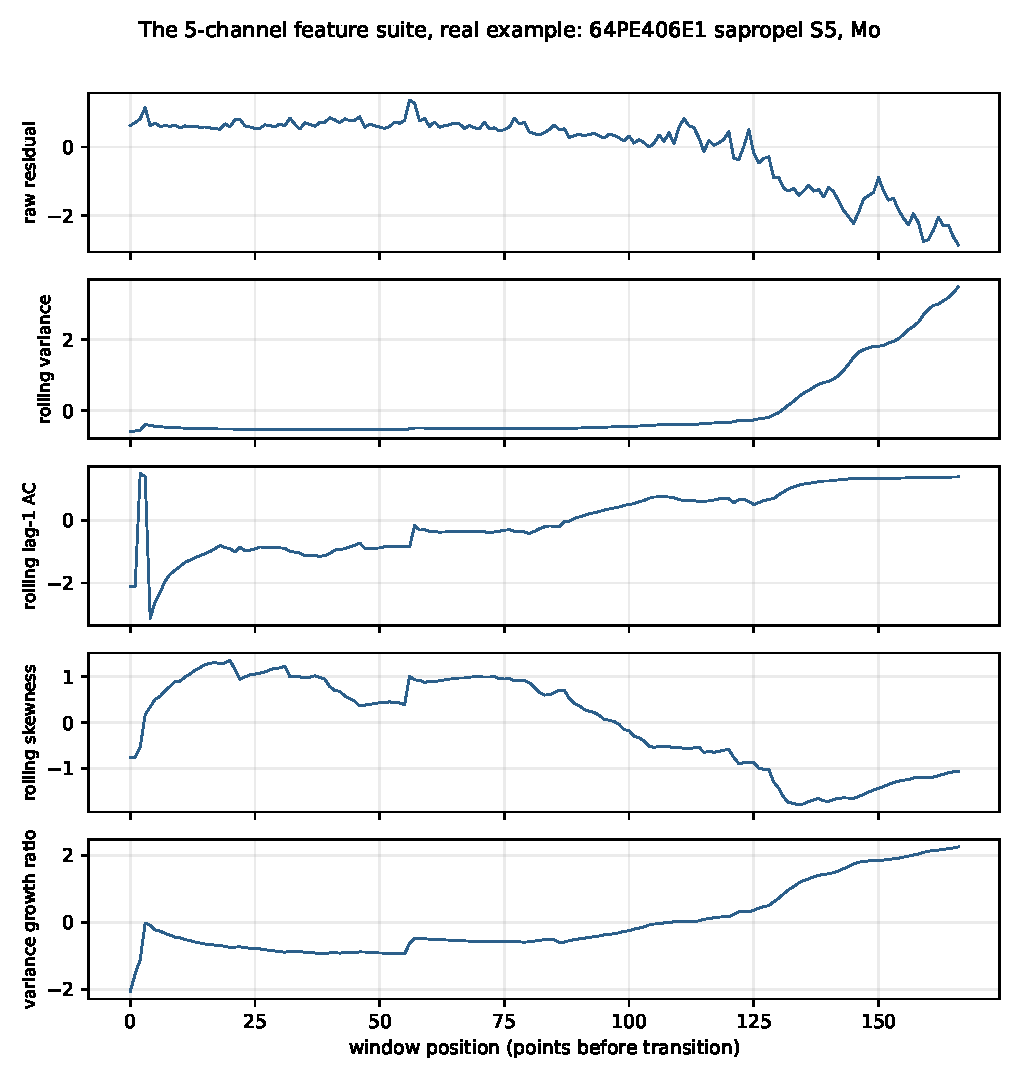
\includegraphics[width=0.72\textwidth]{figures/fig5_feature_channels.pdf}
\caption{The 5-channel feature suite computed on a real example: sapropel S5 in core 64PE406E1, Mo proxy. Only the classical TSC models receive this 5-channel expansion; the deep-learning models read the raw residual alone.}
\label{fig:feature_channels}
\end{figure}

All five channels, for the models that receive them, are z-normalized using statistics computed once on the training set and reused unchanged at test time, so that no information from the test data ever leaks into how a channel is scaled.
